\documentclass[11.5pt,a4paper]{article}
\usepackage[utf8]{inputenc}
\usepackage{amsmath}
\usepackage{amsfonts}
\usepackage{amssymb}
\usepackage{graphicx}
\usepackage{xcolor}
\usepackage[export]{adjustbox}
\usepackage{multicol}
\usepackage[left=2cm,right=2cm,top=2cm,bottom=2cm]{geometry}
\begin{document}

\textbf{\textcolor{gray}{\Huge Mehjebin Mujeeb}}\\ \hrule
%\textbf{\textcolor{gray}{\Huge About}}\\

\t Address: 38/ 2883 Hayath,\\ 
\t PPN Nagar ,Edappally, Kochi\\
\t Email: mehjebin.mujeeb@gmail.com\\
\t phone:+91-9495612744\\
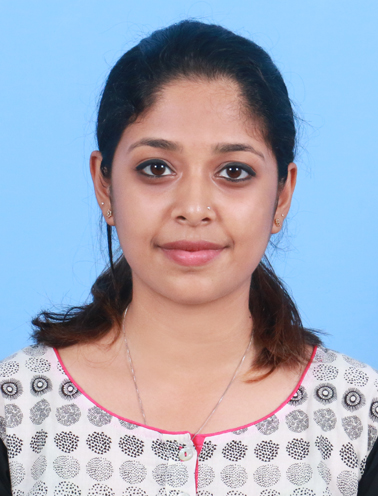
\includegraphics[scale=0.7, width=0.19\textwidth,right ]{pp}



\textbf{\textcolor{gray}{\huge Objective}}\\ \hrule
Seeking an internship position that will allow me to explore career options in the IT sector. A self-motivated, hardworking under-graduate student in computer science looking to improve technical skills.\\

\textbf{\textcolor{gray}{\huge Education}}


\begin{center}
\begin{tabular}{ |c|c|c|c|c| } 
 \hline
 \textbf{\Large Degree} &\textbf{\Large college/School}&\textbf{\Large University} & \textbf{\Large Passing year}& \textbf{\Large Pass \%} \\ \hline
BTech & FISAT,Angamaly & KTU & 2019 & 8.15(cgpa)\\ \hline
XIIth Standard & Army Public School,Pune & CBSE & 2015 & 91\% \\ \hline
Xth Standard & Army Public School,Bangalore & CBSE & 2013 & 9.4(cgpa)\\

 \hline
\end{tabular}
\end{center}

\textbf{\textcolor{gray}{\huge Projects}}\hrule
\begin{itemize}
\item[•] Multinomial Logistic Regression (Design Project)\\
       Domain – Machine learning.
\item[•] Disease Diagnosis Machine (e-Yantra Idea Competition 2018)
\end{itemize}

\textbf{\textcolor{gray}{\huge Training and Internship}}\hrule
\begin{itemize}
\item Android Application Development -\\
Learned to create a basic android app and use Android Studio.
\item Machine Learning course on Udemy
\item Web development bootcamp on Udemy (ongoing)
\end{itemize}

\textbf{\textcolor{gray}{\huge Research Publications}}\\ \hrule
\begin{itemize}
\item[•]None
\end{itemize}


\textbf{\textcolor{gray}{\huge Technical Skills}}\\ \hrule
\begin{itemize}
\item Languages- C, Python, Java, HTML, CSS
\item Database- MYSQL
\item Operating Systems- Windows, Linux
\end{itemize}

\textbf{\textcolor{gray}{\huge Soft Skills}}\\ \hrule
\begin{itemize}
\item Language Lab Training 
\end{itemize}

\textbf{\textcolor{gray}{\huge Strengths}}\\ \hrule
\begin{itemize}
\item Optimistic
\item Hard working
\item Communication (written and verbal) Write and edit reports.
\item Teamwork.
\item Trustworthy 
\item Fast Learner

\end{itemize}

\textbf{\textcolor{gray}{\huge Extra-Curricular Activities}}\\  \hrule
\begin{itemize}
\item Was a part of the Girls BasketBall Team and participated in the inter-college Basket Ball Tournament.
\item Participated in the cultural fest ‘Arangu’ in group dance category.
\item Volunteered for several intra-college as well as IEEE events.
\item Attended The National Conference CSIS  2016 at Trivandrum.
\item Participated in the NACET 2k18 Paper Presentation Competition.

\end{itemize}

\textbf{\textcolor{gray}{\huge Co-Curricular Activities}}\\ \hrule
\begin{itemize}
\item Was part of the special interest group “Centre of Excellence in Robotics and IOT”
\item Participated in e-yantra Robotics Competition 2017
\item Participated in e-yantra Idea Competition 2018-Disease Diagnosis Machine
\item Conducted Several Workshops for Second year student on Arduino

\end{itemize}


\textbf{\textcolor{gray}{\huge Personal Information}}\\ \hrule
\begin{itemize}
\item Father’s Name: Gp. Cpt. V R Mujeeb\\
Occupation: Doctor ( Gastroenterology)
\item Mother’s Name: Sajna Mujeeb\\
Occupation: Home Maker
\item Sibling: Mehreen Mujeeb
\end{itemize}

\textbf{\textcolor{gray}{\huge Reference}}\\ \hrule
\begin{itemize}
\item Mr. Mahesh C\\
 Assistant Professor, CSE\\
           FISAT, Angamaly\\
	 +91-9995286241\\
	 mahesh.fisat@gmail.com\\
	 Mentor for design project\\
\item  Mr. Bejoy Varghese\\
	Assistant Professor (Special Grade), ECE\\
	FISAT, Angamaly\\
	+91-9446029662\\
	bejoyvarghese@fisat.ac.in\\
	Mentor for Disease Diagnosis Machine\\
\item  Dr. Prasad J C\\
	Professor and Head of Department, CSE\\
	FISAT, Angamaly\\
	cheeran.prasad@gmail.com\\
\end{itemize}


\end{document}